% LNCS paper: Mechanistic Interpretability for AI Agent Tool Selection
% Using llncs.cls document class
%
\documentclass[runningheads]{llncs}
%
\usepackage[T1]{fontenc}
\usepackage{graphicx}
\usepackage{amsmath}
\usepackage{amssymb}
\usepackage{bbm}
\usepackage{booktabs}
\usepackage{multirow}
\usepackage{listings}
\usepackage{xcolor}

% Code listing style
\lstset{
  basicstyle=\ttfamily\small,
  breaklines=true,
  frame=single
}

% hyperref loaded last to avoid conflicts with llncs.cls
\usepackage[bookmarks=false,hidelinks]{hyperref}
\renewcommand\UrlFont{\rmfamily}
\urlstyle{rm}
%
\begin{document}
%
\title{Opening the Black Box: Mechanistic Interpretability for AI Agent Tool Selection Using Sparse Autoencoders}
%
\titlerunning{Mechanistic Interpretability for Agent Tool Selection}
%
\author{Hannes Hapke\inst{1}\orcidID{0009-0005-3111-7353} \and
David Cardozo\inst{2}\orcidID{0009-0006-1234-9973}}
%
\authorrunning{H. Hapke and D. Cardozo}
%
\institute{575 Lab, Dataiku Inc., Portland, OR, USA\\
\email{hannes.hapke@dataiku.com}
\and
575 Lab, Dataiku Inc., Toronto, ON, Canada\\
\email{david.cardozo@dataiku.com}}
%
\maketitle
%
\begin{abstract}
AI agents that autonomously select and run tools are increasingly deployed in business contexts, yet their decision-making processes remain opaque. When an agent chooses to query a database rather than search the web, what internal representations drive that choice? Current approaches rely on prompt engineering, behavioral testing, or post-hoc explanations. None of these methods reveal the actual computational mechanisms within the model.

We present a complete mechanistic interpretability pipeline for understanding agent tool-selection decisions. Our approach extracts hidden-state activations from the subject model at the precise moment of tool commitment (the \emph{decision token}), trains a JumpReLU Sparse Autoencoder (SAE) to decompose these activations into monosemantic features, and applies contrastive analysis to identify which features are associated with specific decision patterns. Crucially, the SAE learns the model's natural feature vocabulary without contrastive supervision; contrastive pairs serve only as post-hoc statistical probes.

We validate our feature explanations using token-level fuzzing evaluation adapted from Eleuther AI's autointerp methodology, which tests whether labels identify the correct tokens that activate each feature, not just the correct texts. Our pipeline processes diverse agent scenarios across five domains and produces human-readable decision reports explaining the internal factors driving tool selection. Our implementation is open source at \url{https://github.com/dataiku/kiji-inspector}.

\keywords{Mechanistic interpretability \and Sparse autoencoders \and AI agents \and Tool selection \and Feature interpretation}
\end{abstract}
%
%
%
\section{Introduction}

The deployment of AI agents capable of autonomous tool selection represents a significant advance in artificial intelligence capabilities. Modern agents can access databases, execute code, search the web, and delegate to sub-agents based on natural language requests. However, this capability comes with a fundamental transparency problem: we cannot inspect the internal decision process that leads an agent to choose one tool over another.

Consider an agent that receives the request ``Find information about our company's API rate limits.'' The agent might choose between searching internal documentation or the public web. Understanding \emph{why} the model interprets ``our company's'' as requiring internal search, rather than treating it as a generic reference, requires inspecting the model's internal representations, not just its outputs.

Current approaches to understanding agent behavior fall into three categories, none of which provide mechanistic insight:

\begin{enumerate}
\item \textbf{Prompt engineering}: Modifying system prompts and observing behavioral changes reveals correlations but not causal mechanisms.
\item \textbf{Behavioral testing}: Probing with test inputs characterizes input-output relationships without explaining intermediate computations.
\item \textbf{Chain-of-thought inspection}: Examining generated reasoning text provides a narrative but not the actual computation. Models can produce plausible-sounding explanations that do not reflect their true decision process.
\end{enumerate}

Mechanistic interpretability offers an alternative: directly examining the model's internal representations to identify the computational features that contribute to decisions. Recent work on Sparse Autoencoders (SAEs) has demonstrated that neural network activations can be decomposed into interpretable, monosemantic features that correspond to human-understandable concepts~\cite{ref_bricken2023,cunningham2023sparseautoencodershighlyinterpretable}. However, this work has focused primarily on next-token prediction in language models, not on the structured decision-making that characterizes AI agents.

This paper presents a complete pipeline for mechanistic interpretability of agent tool-selection decisions. Our contributions are:

\begin{enumerate}
\item \textbf{Decision token extraction}: We identify the precise position in the prompt where the model commits to a tool choice and extract activations at this critical moment.
\item \textbf{Contrastive pairs as post-hoc probes}: We generate synthetic pairs of semantically similar requests requiring different tools, but use these pairs only for statistical analysis \emph{after} SAE training. The SAE learns the model's natural feature vocabulary unsupervised. Contrastive pairs are used to identify which of these pre-existing features are associated with specific decision differences.
\item \textbf{JumpReLU SAE with tanh sparsity}: We employ a JumpReLU activation function that produces exact zeros (true sparsity) with learnable per-feature thresholds, trained using a smooth tanh-based sparsity penalty.
\item \textbf{Token-level fuzzing evaluation}: We adapt Eleuther AI's autointerp methodology~\cite{ref_juang2024} to validate whether feature labels correctly identify \emph{which tokens} activate each feature, catching explanations that are ``right for the wrong reasons.''
\end{enumerate}


\section{Related Work}
\label{sec:related}

\subsection{Sparse Autoencoders for Interpretability}

Sparse autoencoders have emerged as a powerful tool for decomposing neural network activations into interpretable features. Bricken et al.~\cite{ref_bricken2023} demonstrated that SAEs trained on language model activations can recover monosemantic features, identifying individual neurons in the SAE that correspond to single, interpretable concepts. This addresses the \emph{superposition hypothesis}, which posits that neural networks represent more features than they have dimensions by encoding multiple concepts in overlapping directions~\cite{elhage2022toymodelssuperposition}.

Cunningham et al.~\cite{cunningham2023sparseautoencodershighlyinterpretable} extended this work with improvements to SAE training, including better initialization strategies and sparsity penalties. The JumpReLU activation function~\cite{ref_rajamanoharan2024} provides exact sparsity (true zeros rather than near-zero values), which improves interpretability by ensuring features are either clearly active or completely inactive.

\subsection{Mechanistic Interpretability}

Mechanistic interpretability aims to reverse-engineer the algorithms implemented by neural networks~\cite{ref_olah2020}. Early work focused on identifying circuits, subgraphs of neurons that implement specific functions~\cite{conmy2023automatedcircuitdiscoverymechanistic}. More recent approaches use dictionary learning to find interpretable directions in activation space~\cite{ref_sharkey2022}.

\subsection{AI Agents and Tool Use}

Tool-augmented language models have become a dominant paradigm for AI agents. Toolformer~\cite{schick2023toolformerlanguagemodelsteach} demonstrated that language models can learn to use tools through self-supervised learning. ReAct~\cite{yao2023reactsynergizingreasoningacting} introduced a framework combining reasoning and acting in language models. Despite rapid progress in agent capabilities, interpretability of agent decisions has received limited attention.

\subsection{Automatic Interpretability}

Labeling features automatically addresses the scalability challenge of mechanistic interpretability. Bills et al.~\cite{ref_bills2023} used language models to generate explanations for individual neurons. Our token-level fuzzing adapts this approach to validate whether feature labels identify the correct \emph{tokens} that activate each feature.

\subsection{Contrastive Methods}

Contrastive methods have proven effective for identifying meaningful directions in representation space. Contrastive activation addition~\cite{turner2024steeringlanguagemodelsactivation} demonstrated that differences between activations for contrasting inputs can be used to steer model behavior. Representation engineering~\cite{zou2025representationengineeringtopdownapproach} extended these ideas to control model outputs. Our approach uses contrastive pairs for post-hoc statistical analysis rather than for training or steering.


\section{Methodology}
\label{sec:methodology}

\subsection{Pipeline Overview}

Our pipeline consists of six sequential steps (see Fig.~\ref{fig:pipeline}):

\begin{enumerate}
\item \textbf{Contrastive pair generation}: Generate synthetic pairs of user requests sharing the same intent but requiring different tools.
\item \textbf{Activation extraction}: Extract hidden-state activations from the subject model at the decision token position.
\item \textbf{SAE training}: Train a JumpReLU sparse autoencoder on the raw activations.
\item \textbf{Contrastive activation analysis}: Use contrastive pairs as post-hoc probes to identify decision-relevant features.
\item \textbf{Feature interpretation}: Label features using an LLM and generate decision reports.
\item \textbf{Fuzzing evaluation}: Validate feature labels through token-level A/B testing.
\end{enumerate}

The pipeline uses two models in separate memory contexts: a generation model (Qwen3-VL-235B-A22B-Instruct-FP8) for pair generation, feature labeling, and fuzzing judgment; and a subject model (NVIDIA Nemotron-3-Nano-30B-A3B-BF16) for activation extraction. The generation model can be replaced with a closed-source API (e.g., GPT-5.2, Claude Sonnet 4.5).

\begin{figure}[t]
\centering
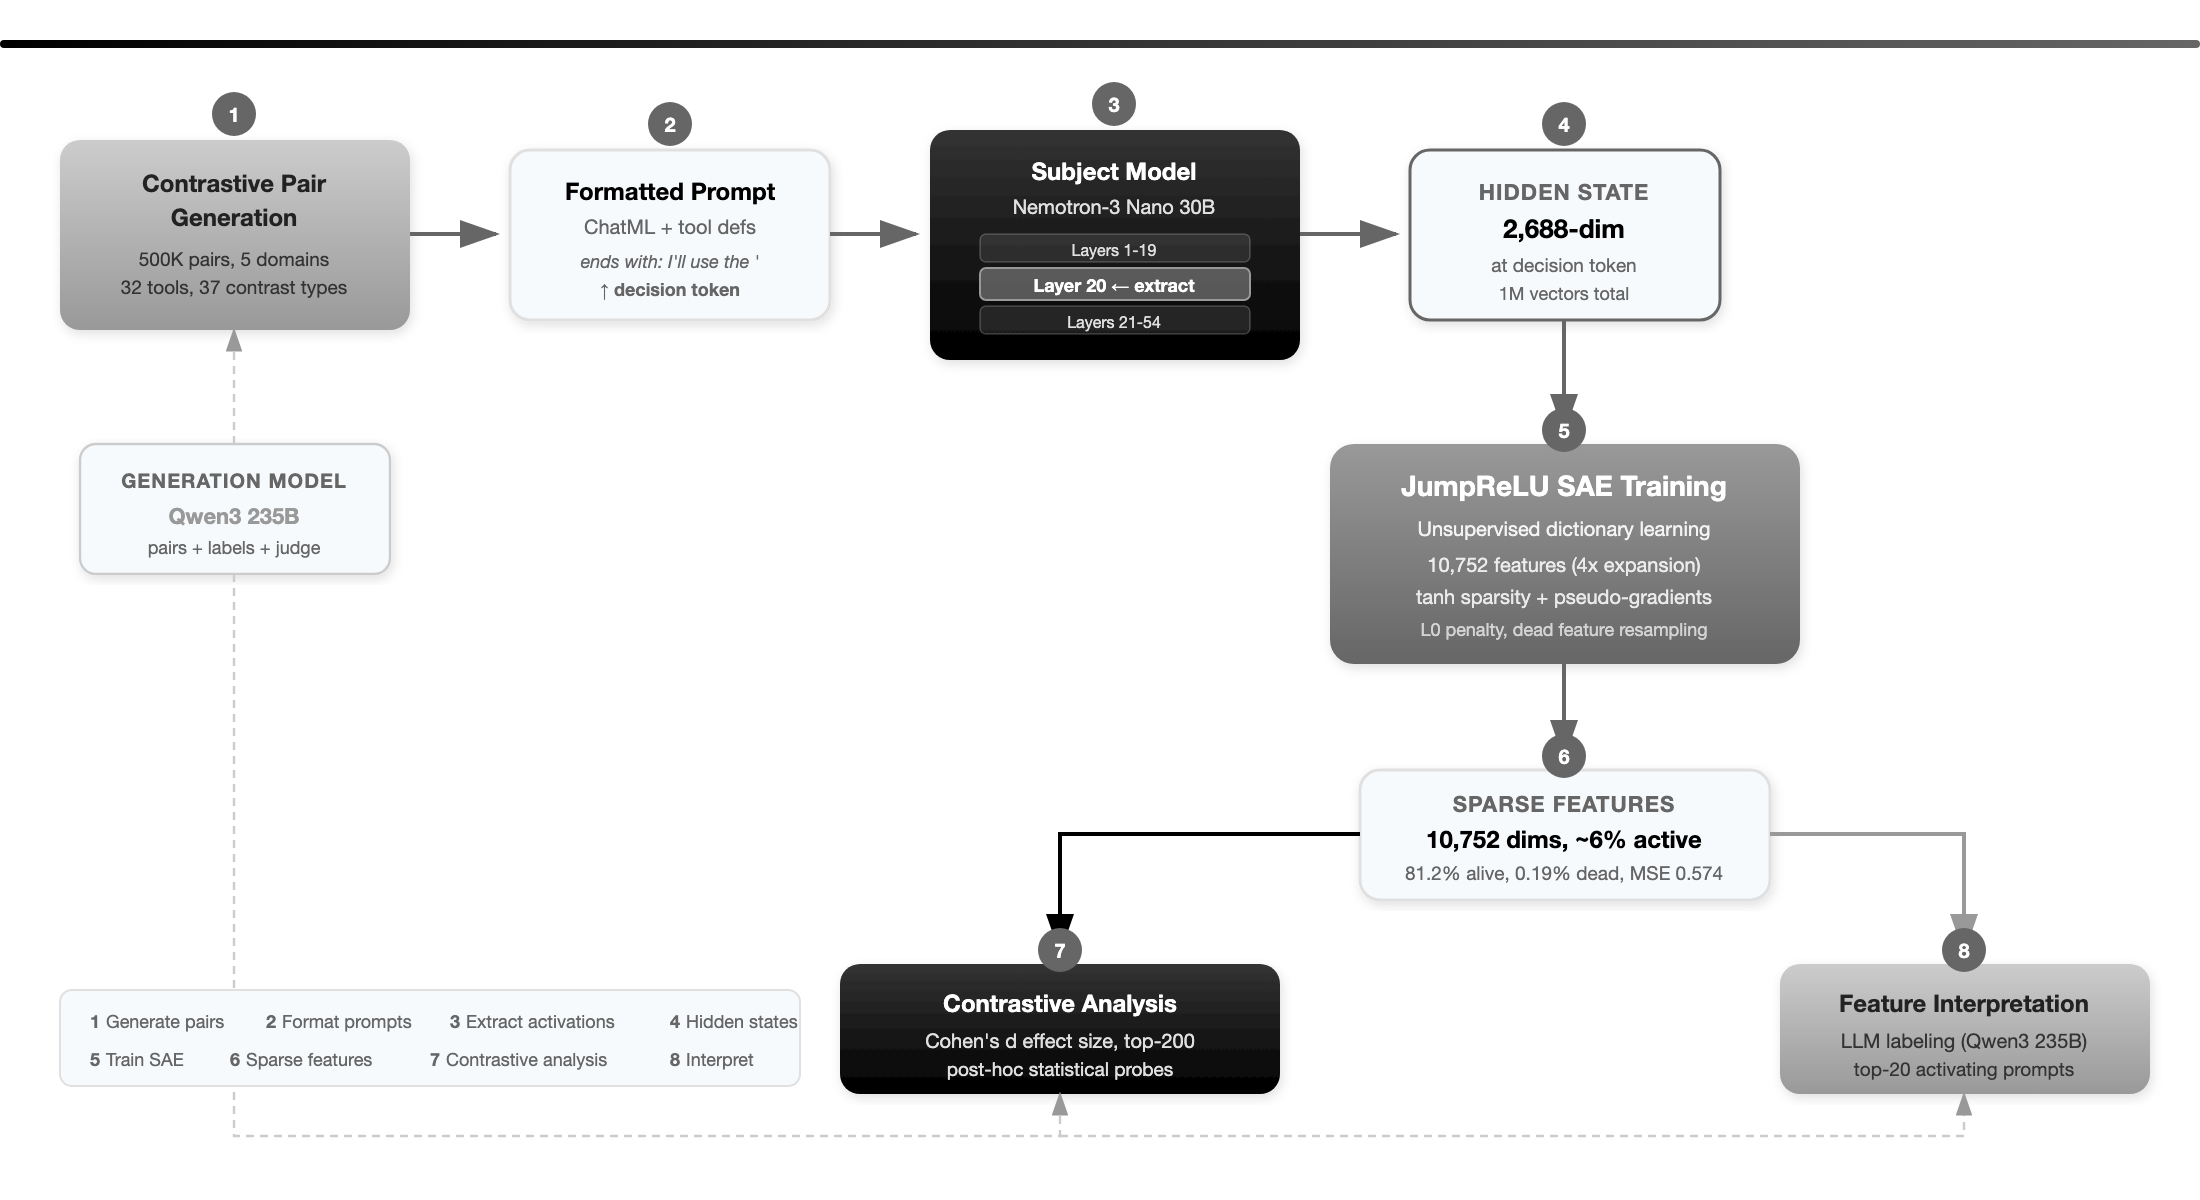
\includegraphics[width=\textwidth]{images/training_pipeline_bw.png}
\caption{Overview of the training pipeline. Contrastive pairs are generated and encoded by the subject model. The SAE is trained unsupervised on the extracted activations; contrastive pairs serve only as post-hoc statistical probes for feature analysis and interpretation.}
\label{fig:pipeline}
\end{figure}

\subsection{Contrastive Pair Generation}

Each contrastive pair captures two semantically similar requests that require different tools. The pair structure includes: anchor prompt, anchor tool, contrast prompt, contrast tool, shared intent, and distinguishing signal.

We define scenarios as JSON configurations specifying a domain (e.g., tool selection, investment analysis), available tools, and contrast types. Table~\ref{tab:scenarios} summarizes the five scenarios in our system.

\begin{table}[t]
\caption{Scenario configurations for contrastive pair generation.}
\label{tab:scenarios}
\centering
\begin{tabular}{llll}
\toprule
Scenario & Tools & Contrast Types & Example Contrast \\
\midrule
tool\_selection & 8 & 13 & read\_vs\_write \\
investment & 6 & 6 & risk\_vs\_return \\
manufacturing & 6 & 6 & quality\_vs\_speed \\
supply\_chain & 6 & 6 & cost\_vs\_reliability \\
customer\_support & 6 & 6 & escalate\_vs\_resolve \\
\bottomrule
\end{tabular}
\end{table}

Pairs are generated using an LLM (Qwen3-VL-235B) with a structured prompt template. The generator includes robust JSON parsing with multiple recovery layers: markdown fence stripping, bracket extraction, trailing comma removal, and truncation recovery. Fuzzy key matching handles LLM variations in JSON field names. Figure~\ref{fig:examples} shows three example pairs from different scenarios.

\begin{figure}[t]
\centering
\begin{lstlisting}[basicstyle=\ttfamily\scriptsize,frame=single,breaklines=true]
Example 1: customer_support (self_service_vs_agent_assist)
Shared Intent: resolve password reset issue
ANCHOR [knowledge_base]: How do I reset my password if I forgot it?
CONTRAST [ticket_lookup]: I tried resetting my password 3 times
                          but the email never arrives.

Example 2: tool_selection (read_vs_write)
Shared Intent: Check latest product version
ANCHOR [file_read]: What is the latest version of Product X?
CONTRAST [file_write]: Set the latest version of Product X to v3.2.1
\end{lstlisting}
\caption{Example contrastive pairs. Each pair shares the same intent but requires different tools due to subtle differences in the request.}
\label{fig:examples}
\end{figure}

\subsection{Decision Token Extraction}

Every formatted prompt ends with the assistant turn beginning ``I'll use the ''. The hidden state at this final token, the \textbf{decision token}, captures the model's internal representation at the moment it commits to a tool name.

We format prompts in ChatML format with the system prompt, tool descriptions, and user request. Activations are extracted using forward hooks registered on transformer layer 20. For the Nemotron-3-Nano-30B model (a Mixture-of-Experts architecture with 30B total parameters, 3B active per token), the hidden dimension is 2,688. Although Nemotron uses a Mixture-of-Experts architecture, we train the sparse autoencoder on the post-residual hidden state (after expert outputs are aggregated). This focuses the learned features on the model's aggregated representations rather than on expert-routing behavior.

Batched extraction uses left-padding to align the decision token across variable-length prompts. Activations are cast to float16 and saved as NumPy shards. Nemotron-3-Nano-30B interleaves Mamba2, GQA Attention, and MoE layers; layer~20 is a GQA Attention layer in the mid-network, preceding the MoE layers that introduce sparse expert routing.

\subsection{JumpReLU SAE Architecture}

Our sparse autoencoder uses the JumpReLU activation function~\cite{ref_rajamanoharan2024}, which produces exact zeros through learnable per-feature thresholds $\boldsymbol{\theta} \in \mathbb{R}^M_+$. Given input activation $\mathbf{x} \in \mathbb{R}^n$, pre-activations are $\boldsymbol{\pi}(\mathbf{x}) = W_\text{enc}(\mathbf{x} - \mathbf{b}_\text{dec}) + \mathbf{b}_\text{enc}$ and feature activations are
\begin{equation}
f_i(\mathbf{x}) = \pi_i(\mathbf{x}) \cdot H(\pi_i(\mathbf{x}) - \theta_i), \qquad \hat{\mathbf{x}}(\mathbf{f}) = W_\text{dec}\,\mathbf{f} + \mathbf{b}_\text{dec},
\end{equation}
where $H$ is the Heaviside step function, $M = 4n$ is the dictionary size, and the decoder bias $\mathbf{b}_\text{dec}$ is shared (subtracted before encoding, added after decoding). Decoder columns are normalized to unit norm after each step.

\paragraph{Loss function.} The loss combines reconstruction with an L0 sparsity penalty:
\begin{equation}
\mathcal{L}(\mathbf{x}) = \|\mathbf{x} - \hat{\mathbf{x}}(\mathbf{f}(\mathbf{x}))\|_2^2 + \lambda \sum_{i=1}^{M} H(\pi_i(\mathbf{x}) - \theta_i).
\end{equation}
Since $H$ is non-differentiable, we use a smooth tanh approximation $\sum_i \text{ReLU}(\tanh((\pi_i - \theta_i)/\varepsilon))$ for the sparsity term during backprop. Gradients with respect to $\theta_i$ follow the kernel-density pseudo-derivatives of Rajamanoharan et al.~\cite{ref_rajamanoharan2024} with rectangular kernel and bandwidth $\varepsilon$; gradients with respect to pre-activations use a standard straight-through estimator.

\begin{figure}[t]
\centering
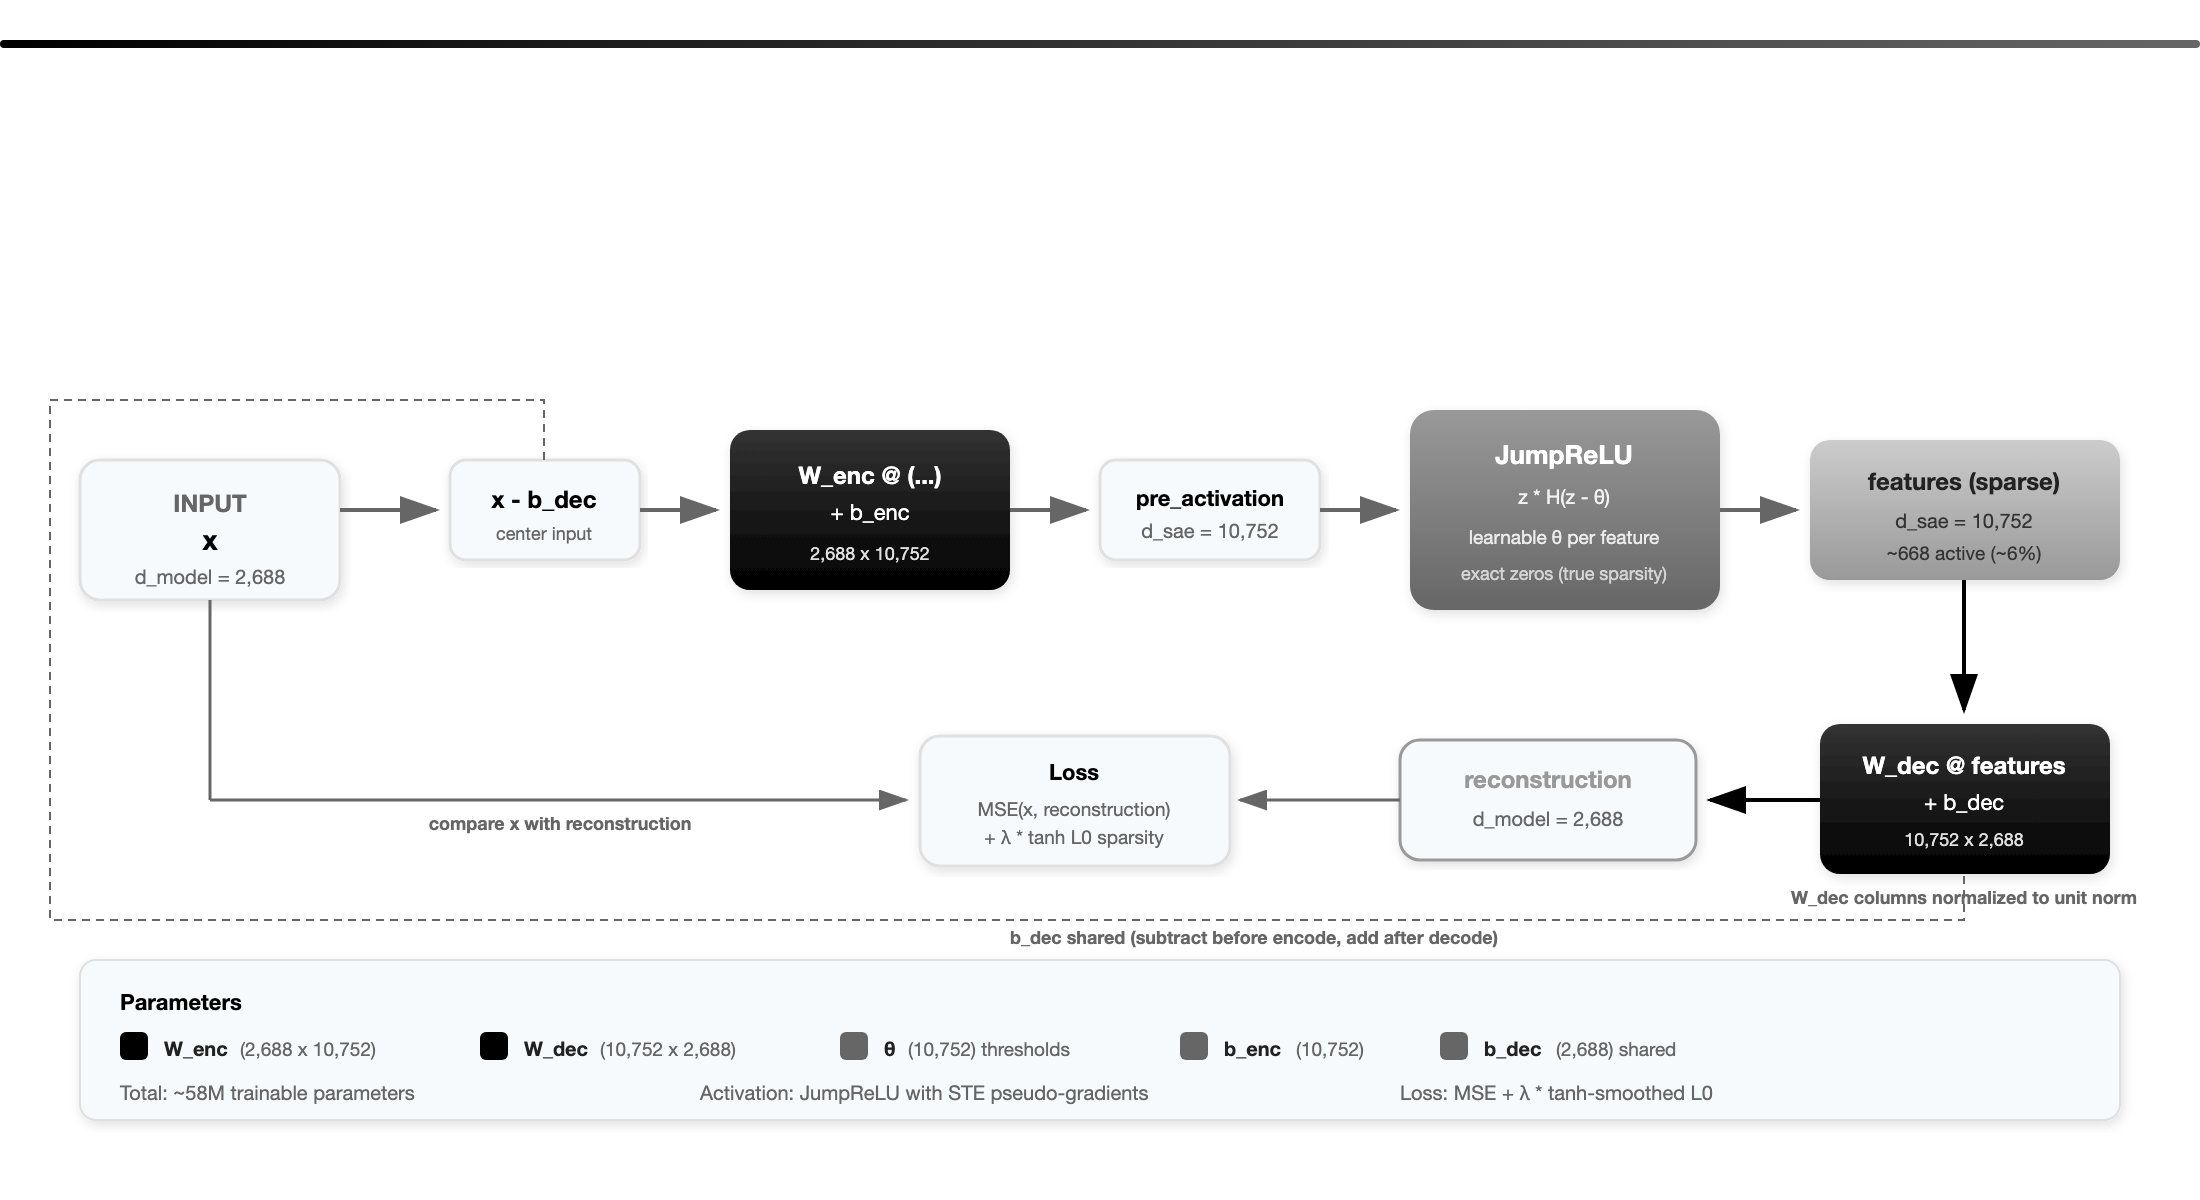
\includegraphics[width=\textwidth]{images/sae_architecture_bw.png}
\caption{JumpReLU Sparse Autoencoder architecture. The input activation $\mathbf{x}$ is centered by subtracting $\mathbf{b}_\text{dec}$, projected to a 10,752-dimensional latent space via $W_\text{enc}$, and sparsified by the JumpReLU activation with learnable thresholds $\boldsymbol{\theta}$. The decoder reconstructs via $W_\text{dec} + \mathbf{b}_\text{dec}$ (shared bias). The loss combines reconstruction MSE with a smooth tanh-based L0 sparsity penalty.}
\label{fig:sae}
\end{figure}

\paragraph{Training details.} Table~\ref{tab:hyperparams} summarizes key hyperparameters. Training uses cosine learning rate decay with linear warmup, sparsity coefficient warmup, and dead feature resampling. Decoder columns are normalized to unit norm after each step.

\begin{table}[t]
\caption{SAE training hyperparameters.}
\label{tab:hyperparams}
\centering
\begin{tabular}{lll}
\toprule
Parameter & Value & Description \\
\midrule
$M$ & 10,752 & Dictionary size ($4\times n$) \\
Batch size & 8,192 & Activations per training step \\
Learning rate & $3 \times 10^{-4}$ & Peak learning rate \\
$\lambda$ & $5 \times 10^{-3}$ & Sparsity coefficient \\
$\varepsilon$ & 0.001 & JumpReLU bandwidth \\
Warmup & 5\% of steps & LR warmup fraction \\
Sparsity warmup & 10\% of steps & Sparsity coefficient warmup \\
Resample interval & 20\% of steps & Dead feature resampling \\
\bottomrule
\end{tabular}
\end{table}

\subsection{Contrastive Feature Analysis}

After SAE training, we identify decision-relevant features using contrastive pairs as post-hoc statistical probes. For each pair, we extract fresh activations and encode through the trained SAE, then compute per-feature statistics.

\paragraph{Cohen's d effect size.} For each feature $j$ across pairs of a contrast type:
\begin{equation}
d_j = \frac{|\bar{f}^{(a)}_j - \bar{f}^{(c)}_j|}{s_\text{pooled}}
\end{equation}
where $\bar{f}^{(a)}_j$ and $\bar{f}^{(c)}_j$ are mean activations for anchor and contrast prompts, and $s_\text{pooled}$ is the pooled standard deviation.

\paragraph{Filtering.} We apply two filters before ranking: effect size $d_j \geq 0.3$ (small-to-medium effect) and minimum activation $\max(|\bar{f}^{(a)}_j|, |\bar{f}^{(c)}_j|) > 0.01$. The top-K features (default: 200) per contrast type are selected for interpretation.

\subsection{Feature Interpretation}

For each decision-relevant feature, we collect the top-20 highest-activating prompts and bottom-10 near-zero prompts from the activation dataset. An LLM (Qwen3-VL-235B) receives these examples and generates a short label (3-8 words), a one-sentence description, and a confidence rating (high/medium/low).


\section{Evaluation: Token-Level Fuzzing}
\label{sec:evaluation}

\subsection{Motivation}

Feature labels may be ``right for the wrong reasons'', correctly predicting which prompts activate a feature but for an incorrect conceptual reason. Token-level evaluation addresses this by testing whether labels identify the specific \emph{tokens} that drive feature activation.

\subsection{Methodology}

\paragraph{Per-token extraction.} Unlike decision-token extraction (single position), fuzzing extracts activations for every token in the prompt, yielding a $(seq\_len, d_\text{model})$ matrix per prompt.

\paragraph{User request span detection.} We locate the user request within the formatted prompt using ChatML structural markers. We highlight only user-request tokens, since highlighting system-prompt or tool-description tokens would be uninformative.

\paragraph{Token highlighting.} For each (prompt, feature) pair: (1) encode per-token activations through the SAE, (2) extract the feature column for the user request span, (3) highlight top-$K$ tokens (adaptive $K$: at most 1/3 of user tokens), and (4) mark with double angle brackets.

\paragraph{A/B comparison.} Token-level examples pair a highlighted top-activating prompt with a highlighted bottom-activating prompt. The A/B order is randomized to prevent position bias. An LLM judge determines which highlighted text better matches the feature label.

\subsection{Metrics}

\paragraph{Combined score.} Token-level accuracy is weighted more heavily:
\begin{equation}
\text{combined} = 0.7 \cdot \text{acc}_\text{token} + 0.3 \cdot \text{acc}_\text{prompt}
\end{equation}

Token-level receives higher weight because it tests the actual mechanism (which tokens trigger the feature), not just text-level correlation.

\paragraph{Quality tiers.} Features are classified by combined score: Excellent ($> 0.8$), Good ($0.6 - 0.8$), Poor ($< 0.6$). Random guessing yields 50\% accuracy (binary A/B choice).


\section{Experimental Setup}
\label{sec:experiments}

\paragraph{Hardware.} Experiments were conducted on a GB200 NVL4 instance with four B200 GPUs (768 GB total GPU VRAM).

\paragraph{Models.} We use two models:
\begin{enumerate}
\item \textbf{Generation/Labeling/Judge}: Qwen/Qwen3-VL-235B-A22B-Instruct-FP8 via vLLM with tensor and expert parallelism.
\item \textbf{Subject model}: nvidia/NVIDIA-Nemotron-3-Nano-30B-A3B-BF16 via HuggingFace Transformers with automatic device mapping.
\end{enumerate}

\paragraph{Scenarios.} We evaluate across five domains with a total of 32 tools and 37 contrast types. The tool\_selection scenario serves as the primary benchmark with 8 general-purpose tools and 13 contrast types.

\paragraph{Dataset scale.} For benchmarking, we generate 500,000 contrastive pairs, yielding 1,000,000 activation vectors.

\paragraph{Layer selection.} To justify our choice of extraction layer, we sweep across layers $\{8, 16, 20, 32, 44\}$ of the 54-layer Nemotron architecture, running steps 2--4 (activation extraction, SAE training, contrastive feature identification) at each depth using a stratified subsample of 5,000 pairs per contrast type.

\section{Results}
\label{sec:results}

\subsection{Layer Sweep}

Table~\ref{tab:layer_sweep} reports SAE quality metrics across five extraction depths. Early layers (8, 16) achieve low reconstruction error but represent pre-decision processing. Mid-network layers (20) balance reconstruction fidelity with decision-relevant representations: layer~20 achieves the highest alive feature percentage (81.2\%) and lowest dead feature rate (0.19\%) while maintaining moderate L0 sparsity. Deep layers (32, 44) exhibit dramatically higher reconstruction MSE ($>$500$\times$ that of layer~20), suggesting the SAE struggles to faithfully capture these representations---likely because layers 32+ in the Nemotron architecture are Mixture-of-Experts (MoE) layers with sparse expert routing, producing activations that are harder to decompose with a single autoencoder.

\begin{table}[t]
\caption{Layer sweep results. SAE quality metrics across transformer depths ($M = 16{,}384$, 5K pairs per contrast type, steps 2--4 only). Layer~20 (bold) is selected for all subsequent experiments.}
\label{tab:layer_sweep}
\centering
\begin{tabular}{rrrrrr}
\toprule
Layer & Alive \% & Dead \% & L0 (mean $\pm$ SEM) & Recon.\ MSE & Features \\
\midrule
8  & 85.3 & 0.10 & $540 \pm 20$   & 0.031   & 192 \\
16 & 63.2 & 0.85 & $539 \pm 13$   & 0.333   & 200 \\
\textbf{20} & \textbf{81.2} & \textbf{0.19} & $\mathbf{668 \pm 26}$ & \textbf{0.574} & \textbf{200} \\
32 & 69.5 & 2.00 & $2{,}231 \pm 11$ & 1{,}524 & 200 \\
44 & 72.0 & 1.01 & $2{,}060 \pm 12$ & 508     & 200 \\
\bottomrule
\end{tabular}
\end{table}

We select layer~20 based on three criteria: (1)~highest alive feature utilization, (2)~lowest dead feature rate, and (3)~reconstruction MSE below 1.0, indicating the SAE faithfully captures the residual stream. While layer~8 has lower MSE, its representations precede the model's tool-selection reasoning; layers 32 and 44 have reconstruction errors three orders of magnitude higher, making their SAE decompositions unreliable.

\subsection{Feature Health Analysis}

Post-training analysis of the layer-20 SAE on the full dataset (1M activation vectors) reveals the distribution of feature activity. Table~\ref{tab:health} summarizes the metrics.

\begin{table}[t]
\caption{SAE feature health metrics (layer~20, full dataset).}
\label{tab:health}
\centering
\begin{tabular}{ll}
\toprule
Metric & Value \\
\midrule
Total features ($M$) & 10,752 \\
Alive features ($>$0.1\% firing rate) & 81.2\% [80.6, 81.8] \\
Dead features (0\% firing rate) & 0.19\% [0.13, 0.27] \\
L0 (mean active features per input) & $668 \pm 26$ (SEM) \\
Reconstruction MSE & 0.574 \\
\bottomrule
\end{tabular}
\end{table}

The 81.2\% alive feature rate indicates that the majority of SAE capacity is utilized, while the L0 statistic confirms sparse encoding (668 active features out of 10,752 total, i.e., 6.2\% activation density).

\subsection{Baseline Comparisons}

To contextualize the SAE's contribution, we evaluate two baselines on the same layer-20 activations (841,282 vectors across 32 tools). Table~\ref{tab:baselines} reports the results.

\begin{table}[t]
\caption{Baseline comparison on raw layer-20 activations (841K vectors, 32 tools). Linear probe uses 5-fold GroupKFold cross-validation; PCA+k-means uses 50 components and 32 clusters.}
\label{tab:baselines}
\centering
\begin{tabular}{lll}
\toprule
Method & Metric & Value \\
\midrule
\multirow{2}{*}{Linear probe} & Accuracy & $0.796 \pm 0.001$ (SEM) \\
 & Macro F1 & $0.765 \pm 0.001$ (SEM) \\
\midrule
\multirow{3}{*}{PCA + k-means} & Purity & 0.175 \\
 & NMI & 0.225 \\
 & ARI & 0.068 \\
\bottomrule
\end{tabular}
\end{table}

A logistic regression on raw activations predicts the correct tool with 79.6\% accuracy across 32 classes, confirming that tool identity is linearly encoded at layer~20. However, this supervised baseline provides no interpretability, it cannot explain \emph{why} a particular tool was chosen. Unsupervised PCA+k-means fails to recover tool structure (NMI~$= 0.225$, ARI~$= 0.068$), indicating that tool-relevant signal is not the dominant source of variance: the first 50 principal components capture only 48\% of total variance, and the resulting clusters do not align with tool boundaries. The SAE bridges this gap by decomposing the same activations into monosemantic features that are both interpretable (91.2\% fuzzing score) and, for select contrast types, causally linked to decisions (Section~\ref{sec:ablation}).

\subsection{Contrastive Feature Discovery}

Contrastive analysis identifies features that systematically differ between anchor and contrast prompts. Top-200 features are selected per contrast type after filtering. A deduplication ratio of 0.7--0.8 indicates moderate feature sharing across contrast types. Top features exhibit Cohen's d $> 0.8$ (large effect).

\subsection{Fuzzing Evaluation}

Table~\ref{tab:fuzzing} summarizes the fuzzing evaluation results across 402 features and 4,422 examples.

\begin{table}[t]
\caption{Fuzzing evaluation results (402 features, 4,422 examples).}
\label{tab:fuzzing}
\centering
\begin{tabular}{ll}
\toprule
Metric & Value \\
\midrule
Features evaluated & 402 \\
Mean combined score & $0.912 \pm 0.008$ (SEM), $p < 10^{-4}$ vs 0.5 \\
Token-level accuracy & $0.906 \pm 0.007$ (SEM), $p < 10^{-4}$ vs 0.5 \\
\midrule
\multicolumn{2}{l}{\textit{Quality tier distribution:}} \\
Excellent ($> 0.8$) & 84.3\% (339 features) \\
Good ($0.6$--$0.8$) & 9.4\% (38 features) \\
Poor ($< 0.6$) & 6.2\% (25 features) \\
\bottomrule
\end{tabular}
\end{table}

Both the combined score and token-level accuracy are significantly above the 50\% random baseline ($p < 10^{-4}$, one-sample $t$-test), with 84.3\% of features achieving excellent quality. Notably, a Kruskal-Wallis test found no significant difference across confidence tiers ($p = 1.0$), indicating the labeling LLM's self-assessed confidence is not predictive of actual fuzzing accuracy in this evaluation.

\subsection{Feature Ablation}
\label{sec:ablation}

To test whether contrastive features are \emph{potentially causally} involved in tool-selection decisions (not merely correlated), we perform a feature ablation experiment. For each contrast type, we intercept the residual stream at layer~20, encode through the SAE, zero out the top-10 contrastive features, decode back, and measure whether the model's tool prediction changes. We include two controls: (1)~ablating 10 random non-contrastive features, and (2)~a \emph{reconstruction-only} baseline that encodes and decodes through the SAE with no features zeroed, measuring distortion from the SAE round-trip alone. Table~\ref{tab:ablation} reports the results for the six contrast types with the highest statistical significance.

\begin{table}[t]
\caption{Feature ablation results (top-10 features ablated, 100 pairs sampled per contrast type). Reconstruction baseline measures SAE round-trip distortion with no features zeroed. Significance via Fisher's exact test (contrastive vs.\ random).}
\label{tab:ablation}
\centering
\small
\begin{tabular}{lrrrrr}
\toprule
Contrast type & $n$ & Contr.\ & Directed & Rand./Recon.\ & $p$ \\
\midrule
fundamental vs.\ technical & 89 & 10.1\% & \textbf{9.0\%} & 0.0\% & \textbf{0.002} \\
single vs.\ multi-tool & 41 & 17.1\% & 2.4\% & 2.4\% & \textbf{0.029} \\
query vs.\ mutate & 9 & 77.8\% & 0.0\% & 33.3\% & 0.077 \\
single-stock vs.\ portfolio & 65 & 10.8\% & 0.0\% & 6.2\% & 0.265 \\
root-cause vs.\ symptom-fix & 15 & 26.7\% & 13.3\% & 13.3\% & 0.326 \\
shallow vs.\ deep & 46 & 8.7\% & 0.0\% & 4.3\% & 0.338 \\
\midrule
\textit{Aggregate (23 types)} & & \textit{16.1\%} & \textit{2.3\%} & \textit{13.0\%} & \\
\bottomrule
\end{tabular}
\end{table}

The strongest evidence of causal involvement emerges for \emph{fundamental vs.\ technical analysis} ($p = 0.002$): ablating contrastive features flips 10.1\% of predictions (9.0\% directed toward the contrast tool), while both random ablation and reconstruction-only produce zero flips. This demonstrates that these specific features are causally necessary for the distinction. A second significant result appears for \emph{single vs.\ multi-tool} ($p = 0.029$), where contrastive ablation produces a 17.1\% flip rate against a 2.4\% baseline.

Critically, the reconstruction-only baseline reveals that the random ablation flip rate equals the SAE round-trip distortion rate across all 23 contrast types, zeroing 10 random features from ${\sim}668$ active features adds no disruption beyond what the encode-decode cycle itself introduces. This validates the experimental design: the SAE reconstruction is sufficiently faithful that ablation effects can be attributed to the specific features removed rather than general signal degradation. For contrast types where no ablation effect is observed (e.g., \emph{preventive vs.\ reactive maintenance}, $n = 95$, 0\% across all conditions), the model's tool-selection decision is robust to removing any 10 features, suggesting these decisions rely on distributed representations rather than sparse feature circuits.


\section{Discussion}
\label{sec:discussion}

\subsection{Key Findings}

The trained SAE decomposes tool-selection activations into features that correspond to human-understandable concepts. Features like ``internal knowledge retrieval,'' ``data modification intent,'' and ``query complexity'' emerge without explicit supervision, and token-level fuzzing confirms that 84.3\% achieve excellent quality ($> 0.8$ combined score), with the aggregate score of $0.912 \pm 0.008$ significantly exceeding the random baseline ($p < 10^{-4}$). Prompt-level accuracy alone would overestimate this quality: some features achieve high prompt-level but poor token-level accuracy, indicating labels that capture text-level correlations without identifying the actual triggering tokens. The same pipeline architecture applies across five diverse scenarios (tool selection, investment, manufacturing, supply chain, customer support), demonstrating generalizability.

Feature ablation demonstrates that contrastive features are causally involved in specific decisions: for \emph{fundamental vs.\ technical analysis}, zeroing the top-10 features flips 10.1\% of predictions (9.0\% directed) while random ablation and reconstruction-only produce zero flips ($p = 0.002$). However, this causal link is contrast-type-dependent---for 9 of 23 tested types, no ablation produces any flips, indicating distributed rather than sparse-circuit representations. The reconstruction-only baseline proved essential: random ablation flip rates match SAE round-trip distortion exactly, confirming that observed effects are attributable to specific feature removal.

At inference time, the trained SAE integrates directly into the agent's forward pass: the layer-20 hidden state is intercepted, projected through the SAE, and the top-K active dimensions are mapped to pre-computed feature labels, producing a human-readable decision report alongside the agent's tool selection. We demonstrate this end-to-end in an interactive demo that surfaces SAE-derived rationales (e.g., inventory tracking, risk alerts) alongside the agent's output.

\subsection{Limitations}

\paragraph{Compute requirements.} The pipeline requires substantial GPU resources: a 235B parameter model for generation/labeling/judging and a 30B parameter subject model for activation extraction.

\paragraph{Label quality depends on labeling LLM.} Feature interpretation relies on the labeling model's ability to identify patterns in max-activating examples. Labeling errors propagate to the decision report.

\paragraph{Coverage of decision factors.} Contrastive pairs are generated synthetically and may not cover all factors that influence tool selection in real deployments.

\paragraph{Ablation scope.} Our ablation experiment zeroes the top-10 contrastive features out of ${\sim}668$ active features per input. For contrast types where this produces no effect, the decision may depend on a larger set of features acting in concert. Ablating more features risks general disruption that confounds causal attribution, while ablating fewer reduces statistical power. The optimal ablation set size remains an open question.

\subsection{Future Work}

Several directions follow directly from these results. \emph{Higher-fidelity SAEs}---via larger dictionaries, improved architectures such as Gated SAEs~\cite{rajamanoharan2024improvingdictionarylearninggated}, or per-layer optimization---would reduce the 13\% reconstruction-only flip rate and enable cleaner causal experiments with larger ablation sets. \emph{Multi-layer analysis} could reveal how tool-selection features emerge and transform across the network, and whether the MoE layers (32+) are better captured by expert-specific decompositions. \emph{Cross-model transfer} experiments (Nemotron to Llama or Qwen) would establish whether tool-selection circuits are architecture-dependent. Finally, integrating the pipeline into production agent systems could provide \emph{real-time decision explanations and anomaly detection}, flagging when feature activations deviate from expected patterns for a given tool choice.


\section{Conclusion}
\label{sec:conclusion}

We have presented a complete mechanistic interpretability pipeline for understanding AI agent tool-selection decisions. By extracting activations at the precise moment of tool commitment, training sparse autoencoders to decompose these activations into interpretable features, and validating explanations through token-level fuzzing, we provide insight into the internal factors driving agent decisions.

Our key methodological contributions include: (1) decision token extraction for capturing the moment of tool commitment; (2) contrastive pairs as post-hoc probes rather than training signals; (3) JumpReLU SAE with tanh sparsity for exact zeros and smooth gradients; and (4) token-level fuzzing evaluation that catches explanations which are ``right for the wrong reasons.''

As AI agents are deployed in increasingly high-stakes contexts, understanding \emph{how} they make decisions, not just \emph{what} decisions they make, becomes critical for safety, debugging, and trust.


\begin{credits}
\subsubsection{\ackname}
This work was conducted as part of Dataiku's 575 Lab, the company's open source office.
The source code for this project is available at \url{https://github.com/dataiku/kiji-inspector}.

\subsubsection{\discintname}
Hannes Hapke and David Cardozo are employees of Dataiku Inc, and part of Dataiku's 575 Lab, the open source office. Compute resources for this project have been provided by NVIDIA, Inc.
\end{credits}

\bibliographystyle{splncs04}
\bibliography{references}

\end{document}
